%TCIDATA{LaTeXparent=0,0,relatorio.tex}
\ifx\compilewholereport\undefined
	\documentclass[11pt,a4paper,oneside]{book}
	
	% Escolher um dos seguintes formatos:
	\usepackage{ft2unb} % segue padrão de fontes do Latex
	
	% Pacotes
	\usepackage{graphicx}
	\usepackage{amsfonts}
	\usepackage{amsmath}
	\usepackage{amssymb}
	\usepackage[thmmarks,amsmath]{ntheorem}
	\usepackage{boxedminipage}
	\usepackage{theorem}
	\usepackage{fancybox}
	\usepackage{fancyhdr}
	\usepackage{url}
	\usepackage{afterpage}
	\usepackage{color}
	\usepackage{colortbl}
	\usepackage{rotating}
	\usepackage{makeidx}
	\usepackage{indentfirst}
	\usepackage{bibentry}
	\usepackage{subcaption}
	\usepackage{todonotes}
	\presetkeys{todonotes}{inline}{}
	
	\begin{document}
	\frontmatter
	\tableofcontents
	\mainmatter
	
	%%%%%%%%%%%%%%%%%%%%%%%%%%%%
	%%%%%%%% Apagar coisas acima
	%%%%%%%%%%%%%%%%%%%%%%%%%%%%
	\newcommand\qt[1]{\lq\lq{}#1\rq\rq{}}
	\newcommand\qti[1]{\lq\lq{}\textit{#1}\rq\rq{}}
\fi

\chapter{Introdu\c{c}\~ao Histórica}\label{CapIntro}

\resumodocapitulo{Este cap\'itulo contextualiza o tema apresentado, apresentando a motivação histórica para o desenvolvimento do mesmo.}

\vspace{0.8cm}
O mundo atual \'e controlado quase que completamente por sistemas digitais.
As informa\c{c}\~oes obtidas pelos sensores s\~ao digitalizadas antes de serem tratadas.
Tal processo de digitaliza\c{c}\~ao \'e importante, visto que elimina os ru\'idos intr\'insecos ao processamento anal\'ogico \cite{chen2004electrical}.

O primeiro computador de computa\c{c}\~ao gen\'erica surgiu por volta da d\'ecada de 40.
Sua inven\c{c}\~ao iniciou a terceira revolu\c{c}\~ao industrial, conhecida como revolu\c{c}\~ao da informa\c{c}\~ao ou revolu\c{c}\~ao t\'ecnico-cient\'ifica-informacional \cite{patterson2005coa}.
Os computadores dessa \'epoca liam e executavam instru\c{c}\~oes de forma linear, em um modelo conhecido como sequencial ou temporal. 

Nos anos que se seguiram, a substituição das válvulas por transistores de sil\'icio ajudaram a reduzir o tamanho dos computadores de metros a cent\'imetros quadrados.
Tal mudan\c{c}a permitiu um aumento na popularidade destes dispositivos para o uso pessoal, efeito que impulsionou a ind\'ustria de produ\c{c}\~ao de processadores \cite{Hennessy2011}.
As empresas da \'epoca come\c{c}aram ent\~ao a guerra de miniaturiza\c{c}\~oes de transistores, marcada pelo c\'elebre artigo de Gordon E. Moore, cofundador da Intel, que dizia que o n\'umero de transistores dentro de um processador duplicaria aproximadamente a cada 2 anos \cite{Moore1965}.
A partir de 1970, a lei foi adaptada para a duplica\c{c}\~ao a cada 18 meses.
A figura \ref{fig:moores_law} apresenta uma visualização da lei de Moore nos anos que se seguiram.

\begin{figure}[h]
	\centering
	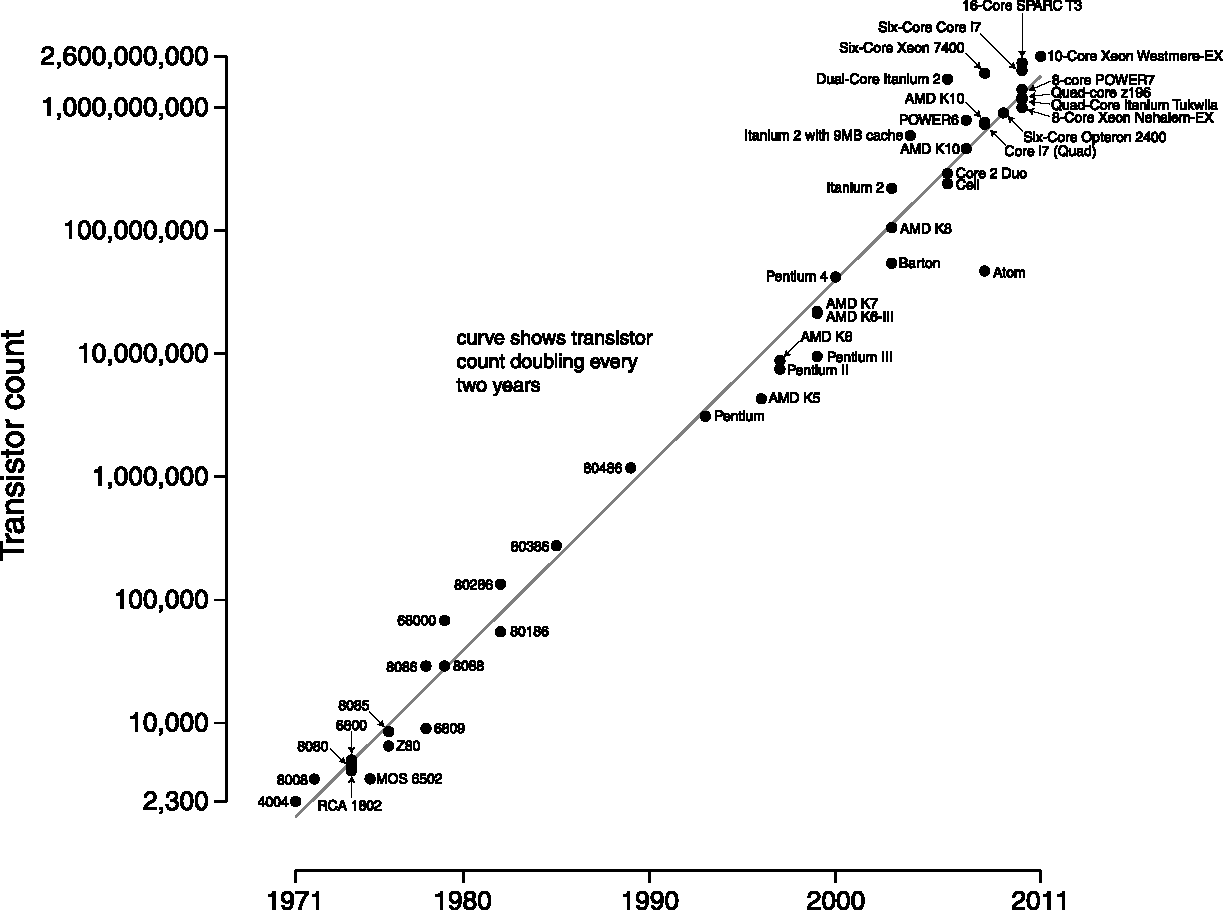
\includegraphics[width=0.7\textwidth]{fig/c1_introducao/moores_law.pdf}
	\caption{Visualização da Lei de Moore. Eixos em escala logarítmica. Extraido de \cite{moore2011}.}
	\label{fig:moores_law}
\end{figure}

Com a integra\c{c}\~ao de mais componentes dentro do processador, conjuntos de instru\c{c}\~oes cada vez mais complexas foram desenvolvidas.
Estas intru\c{c}\~oes surgiram para acelerar a computa\c{c}\~ao de fun\c{c}\~oes de n\'iveis mais altos.
A integra\c{c}\~ao tamb\'em reduziu a pot\^encia dissipada por transistor, permitindo que as frequ\^encias de opera\c{c}\~ao dos computadores fosse aumentada \cite{Hennessy2011}.

Com o aumento da complexidade das instruções, passou-se a adotar duas nomenclaturas diferentes para processadores: \textit{Reduced Instruction Set Computer} (RISC) e \textit{Complex Instruction Set Computer} (CISC) \cite{Fedeli2003}.
A arquitetura RISC possui um conjunto pequeno e muito otimizado de funções, comandos exclusivos para acesso a memória (arquitetura \textit{load/store}) e uma média de uma instrução completada por ciclo, quando desconsidera-se as instruções de acesso a memória.
A arquitetura CISC possui várias funções para tarefas mais específicas, que por vezes demandam vários ciclos de relógio, e funções que realizam operações com informações lendo e/ou salvando direto na/para a memória.
A arquitetura RISC, que possui em seu portfolio dispositivos como ARM, IBM PowerPC, Sun SPARK e MIPS, dentre outros, é muito mais utilizada nos dias de hoje.
A figura \ref{fig:history_risc} mostra um pouco da história desta arquitetura.
Até empresas como a Intel, que ficaram populares com seus processadores CISC, tem se curvado a arquitetura RISC devido a seu uso mais eficiente de potência.
Eles vem utilizando uma arquitetura conhecida como núcleo de RISC (\textit{RISC core}), onde as instruções são recebidas em formato CISC e decodificadas para uma arquitetura interna RISC.

\begin{figure}[h]
\centering
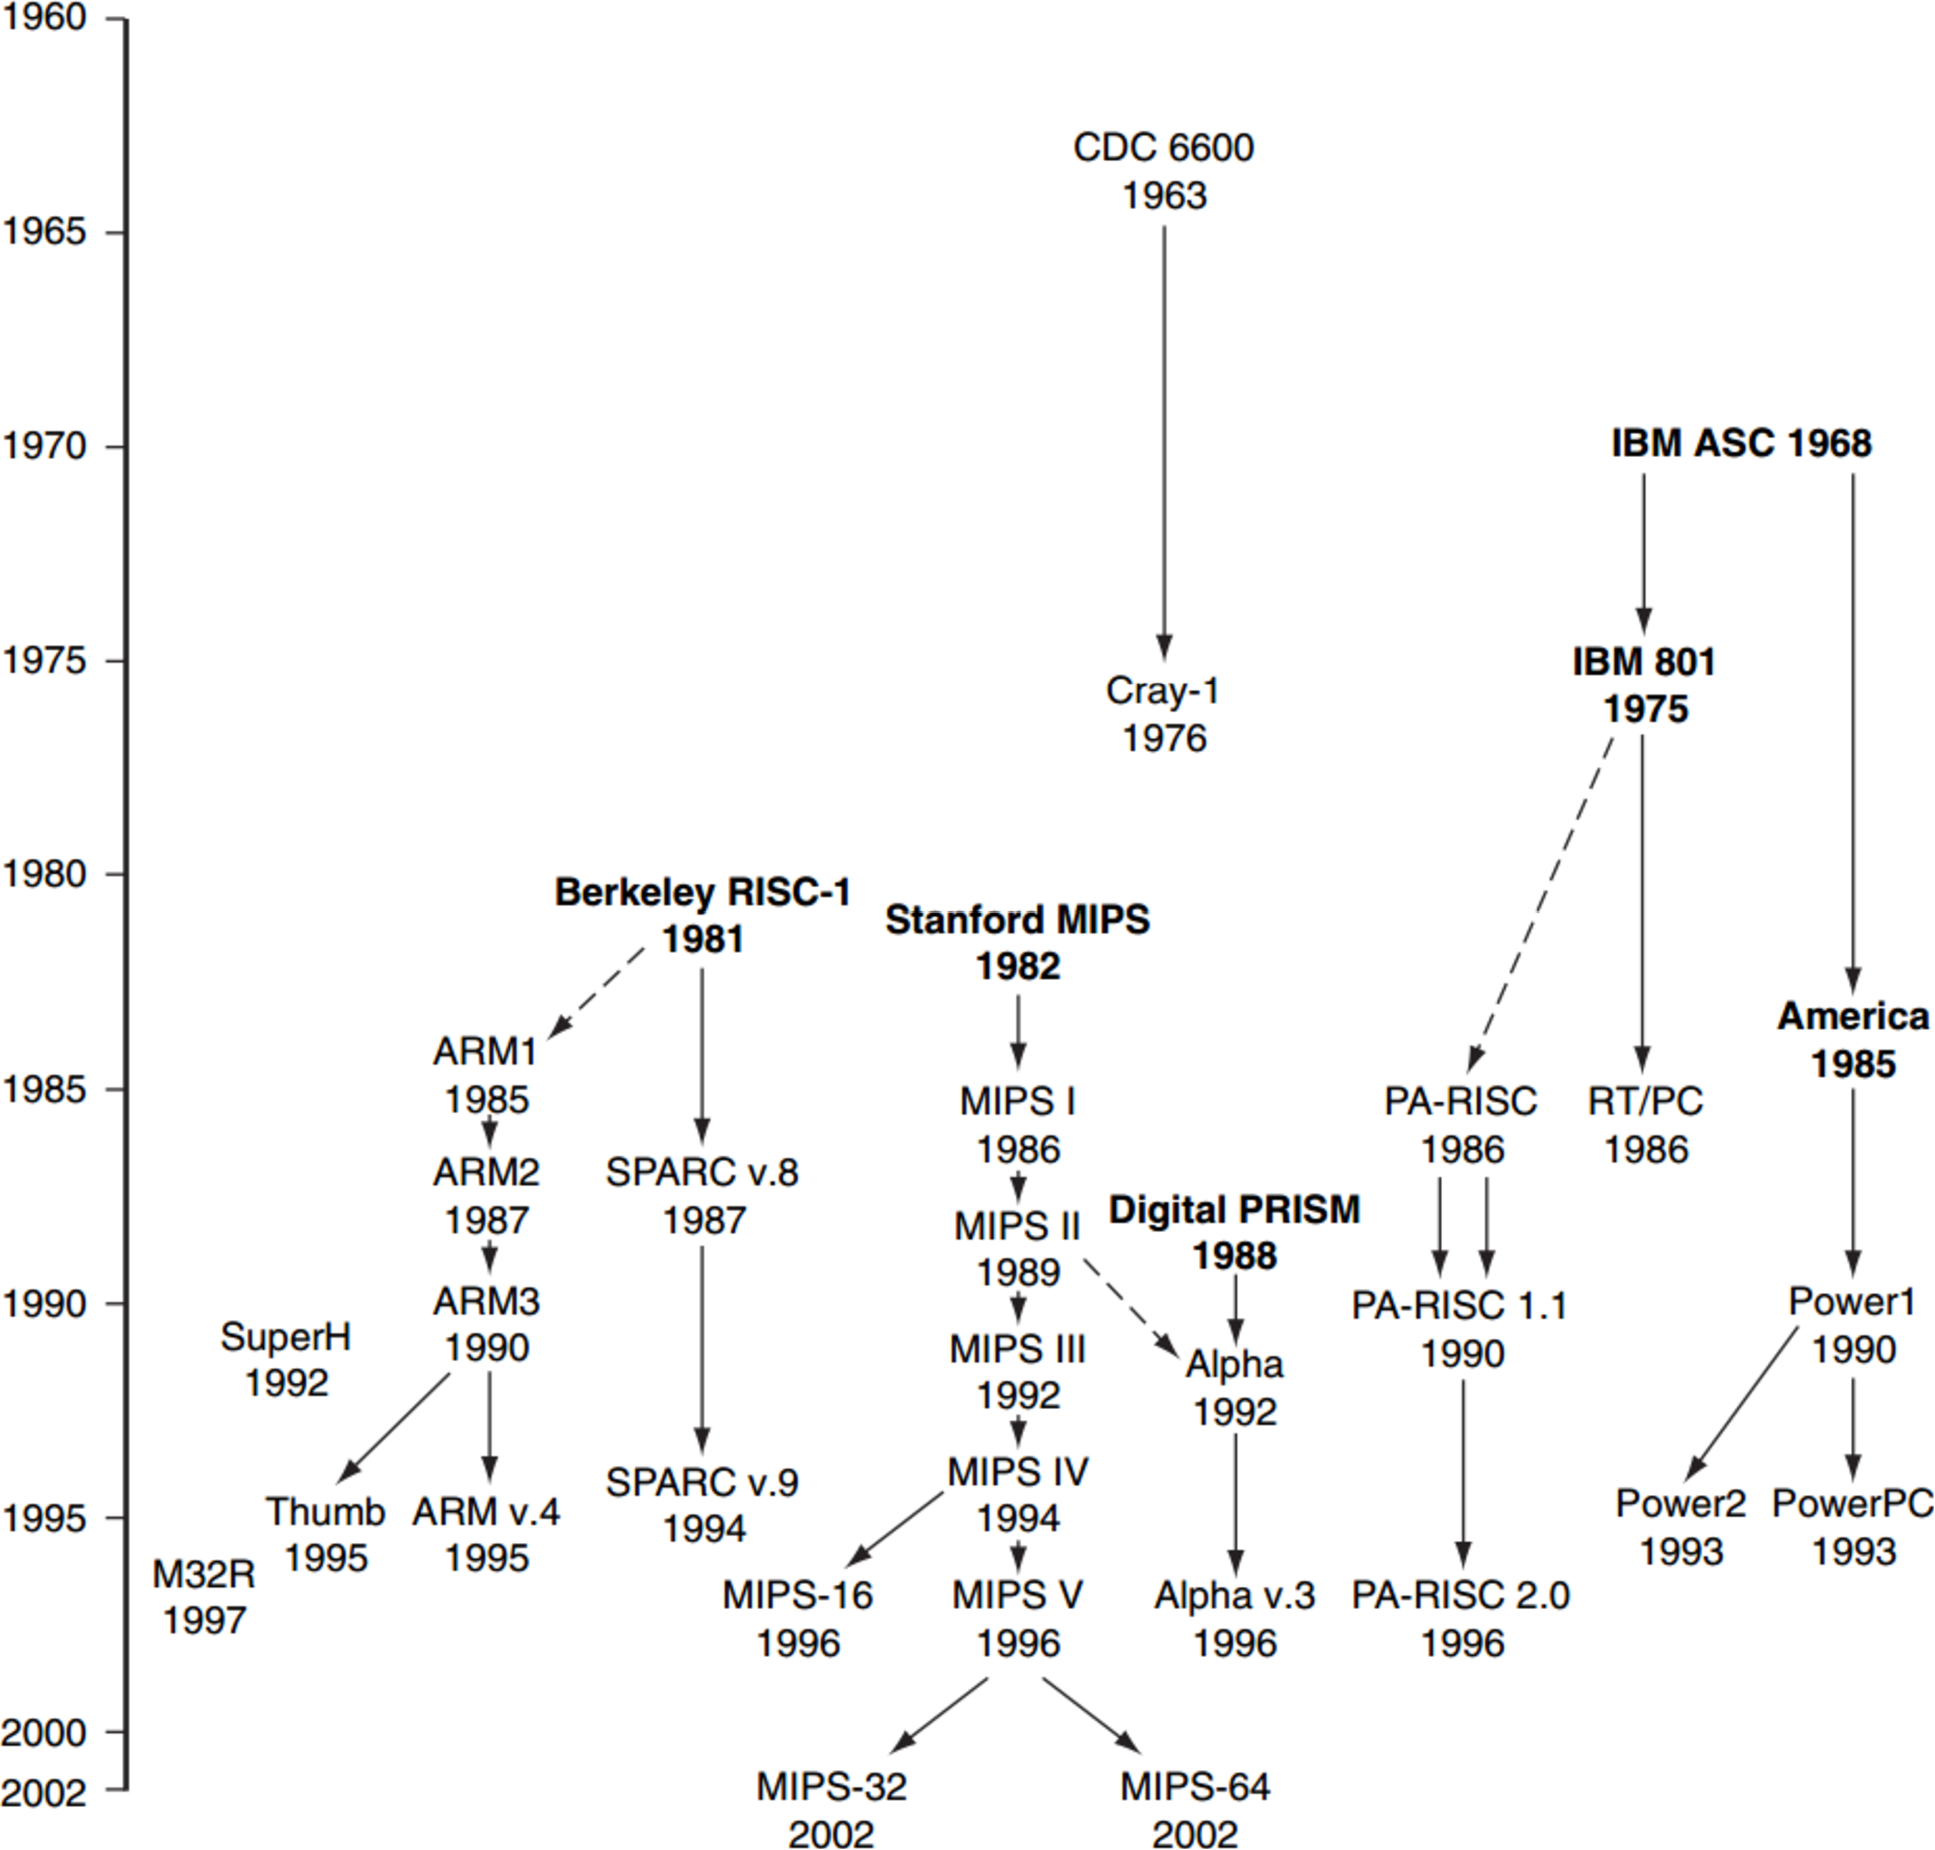
\includegraphics[width=0.7\textwidth]{fig/c1_introducao/history_risc.pdf}
\caption{Linha do tempo das arquiteturas RISC, extraido de \cite{Hennessy2011}. Em negrito estão as iniciativas de pesquisa, em contraste às comerciais.}
\label{fig:history_risc}
\end{figure}

Por volta dos anos 2000, a pot\^encia dissipada em cada transistor, proporcional a frequência de opera\c{c}\~ao, havia atingido o limite suportado pelo microprocessador.
Por causa disso, o crescimento desenfreado da frequ\^encia teve que ser repensado.
Come\c{c}ou-se ent\~ao o desenvolvimento de microprocessadores \textit{multicore}, que aumentam a vaz\~ao de instru\c{c}\~oes (\textit{throughtput}) sem modificar o tempo de resposta, que corresponde ao tempo de processamento médio de uma instrução.
Em meados de 2006, todas as grandes companhias j\'a possuiam produtos com esta arquitetura \cite{Hennessy2011}.

Os microprocessadores com v\'arios n\'ucleos (\textit{multicore}) abriram espa\c{c}o para a chegada de processadores com muitos n\'ucleos (\textit{manycore}).
Estes microprocessadores s\~ao projetados para placas gr\'aficas e, apesar de possuirem centenas de n\'ucleos, estes núcleos s\~ao simplificados \cite{Vajda2011}.
Em geral, eles são capazes de realizar apenas algumas poucas operações, mas abrem caminho para paradigmas de programação que transformem a computação concorrente em computação paralela \cite{Harel2004}.

Mesmo trabalhando com um ou v\'arios n\'ucleos de processamento, o modelo de computa\c{c}\~ao atual ainda \'e dito temporal ou sequencial uma vez que blocos de instru\c{c}\~oes s\~ao executados em seu devido instante de tempo de forma sequencial, conceito destacado pela atomicidade estudada em programa\c{c}\~ao paralela \cite{williams2012c++}.

Do ponto de vista da programa\c{c}\~ao, os primeiros computadores apresentavam programas que n\~ao podiam ser alterados.
Parte desta limita\c{c}\~ao era justificada pela programa\c{c}\~ao utilizando-se cart\~oes, mas nas primeiras gera\c{c}\~oes de computadores com mem\'orias eletr\^onicas o mesmo sistema foi utilizado.

A arquitetura de von Neumann, utilizada na primeira gera\c{c}\~ao de computadores eletr\^onicos, era cons\-ti\-tu\'i\-­da de uma \'unica unidade de mem\'oria, uma unidade de processamento e um canal de comunica\c{c}\~ao.
Esta arquitetura possui tanto uma vantagem tremenda, a capacidade de modifica\c{c}\~ao de programas em tempo de execu\c{c}\~ao, quanto uma falha crucial, conhecida por gargalo de von Neumann.
A vantagem aparece uma vez que, como n\~ao h\'a distin\c{c}\~ao entre mem\'oria de programa e dados, uma instru\c{c}\~ao pode sobrescrever um endere\c{c}o de mem\'oria marcado como programa.
O problema diz respeito \`as restri\c{c}\~oes impostas pelo canal de comunica\c{c}\~ao, que permitia que apenas uma palavra, seja de programa ou de dados, fosse mandada para a unidade de processamento e de volta \cite{Backus1978}.
Este problema se agrava a medida que o processador fica mais r\'apido que a mem\'oria, uma vez que o tempo de espera, em ciclos de rel\'ogios, para a obten\c{c}\~ao da informa\c{c}\~ao aumenta.
Para solucionar o problema do gargalo de von Neumann, a arquitetura Harvard foi proposta.

A arquitetura Harvard original propunha que a mem\'oria de programa e a mem\'oria de dados fossem fisicamente separadas e possuissem cada uma seu pr\'oprio canal de comunica\c{c}\~ao com o processador.
Essa modifica\c{c}\~ao acelera a execu\c{c}\~ao de certos programas, visto que programa e dados podem ser carregados das suas respectivas mem\'orias simultaneamente.
Uma pequena altera\c{c}\~ao na arquitetura Harvard, conhecida de arquitetura Harvard modificada, permitia que mais de um canal de comunica\c{c}\~ao ligasse a uma mem\'oria tanto de programa quanto de dados.
Essas informa\c{c}\~oes eram divididas em mem\'orias tempor\'arias (\textit{cache}) espec\'i­ficas para o programa e para dados, formando assim uma arquitetura Harvard original.
Essa modifica\c{c}\~ao combina os benef\'i­cios da arquitetura de von Neumann, ou seja, a modifica\c{c}\~ao de programas em tempo de execu\c{c}\~ao, e da arquitetura Harvard original, ou seja, o tempo de acesso reduzido.

Atualmente, nossos modernos computadores multiprocessados utilizam a arquitetura Harvard modificada com diversos n\'i­veis de mem\'oria \textit{cache} \cite{Hennessy2011}, sejam eles dedicados ou compartilhados entre os v\'arios processadores.
A sua capacidade de processamento atinge n\'i­veis extraordin\'arios, ultrapassando 20 GFlops em computadores comuns \cite{MaxxPI2013} e 54 PFlops em supercomputadores \cite{Top5002013}.
Apesar disso, a arquitetura Harvard original ainda \'e muito usada em microcontroladores e processadores digitais de sinal (\textit{Digital Signal Processors} ou DSPs).

\section{Computa\c{c}\~ao Reconfigur\'avel}
\label{ss:computacao_reconfiguravel}

A computa\c{c}\~ao reconfigur\'avel foi proposta por volta de 1960 por Gerald Estrin para resolver problemas que n\~ao podiam ser resolvidos pela computa\c{c}\~ao da \'epoca \cite{Estrin2002}.
Estrin prop\^os um microprocessador composto de uma parte fixa e uma parte vari\'avel, onde a parte vari\'avel seria usada para programar funcionamentos espec\'i­ficos para serem usados em determinados per\'i­odos de tempo.
A id\'eia de Estrin foi deixada de lado \`a medida que os microprocessadores e \textit{Application-Specific Integrated Circuits} (ASICs) se mostraram aptos a resolver os problemas da \'epoca.
Por volta da d\'ecada de 1990, por\'em, o primeiro microprocessador h\'i­brido comercial foi desenvolvido \cite{Estrin2002}, trazendo novamente esta tecnologia \`a tona.

A tecnologia inventada por Estrin, tamb\'em conhecida como estrutura \textit{Fixed Plus Variable} (F+V), cuja representação está mostrada na figura \ref{fig:model_f+v}, trouxe \`a tona um novo paradigma de processamento de dados \cite{Hartenstein2001}.
O motivo para tal \'e o fato de que a intera\c{c}\~ao entre as unidades de processamento e os dados mudou completamente.
O que antes se conhecia por modelo temporal de computa\c{c}\~ao foi deixado de lado para, nesta nova arquitetura, se tornar um modelo espacial.
Em outras palavras, os dados n\~ao eram direcionados um a um para uma unidade central de processamento, mas processados continuamente em um sistema distribu\'i­do no espa\c{c}o \cite{vassiliadis2007fine}.
Tal sistema distribu\'i­do \'e composto de c\'elulas l\'ogicas e suas conex\~oes, ambas reprogram\'aveis, ajudando a se alcan\c{c}ar uma efici\^encia similar a presente em ASICs e flexivel como a computa\c{c}\~ao gen\'erica.

\begin{figure}[h]
\centering
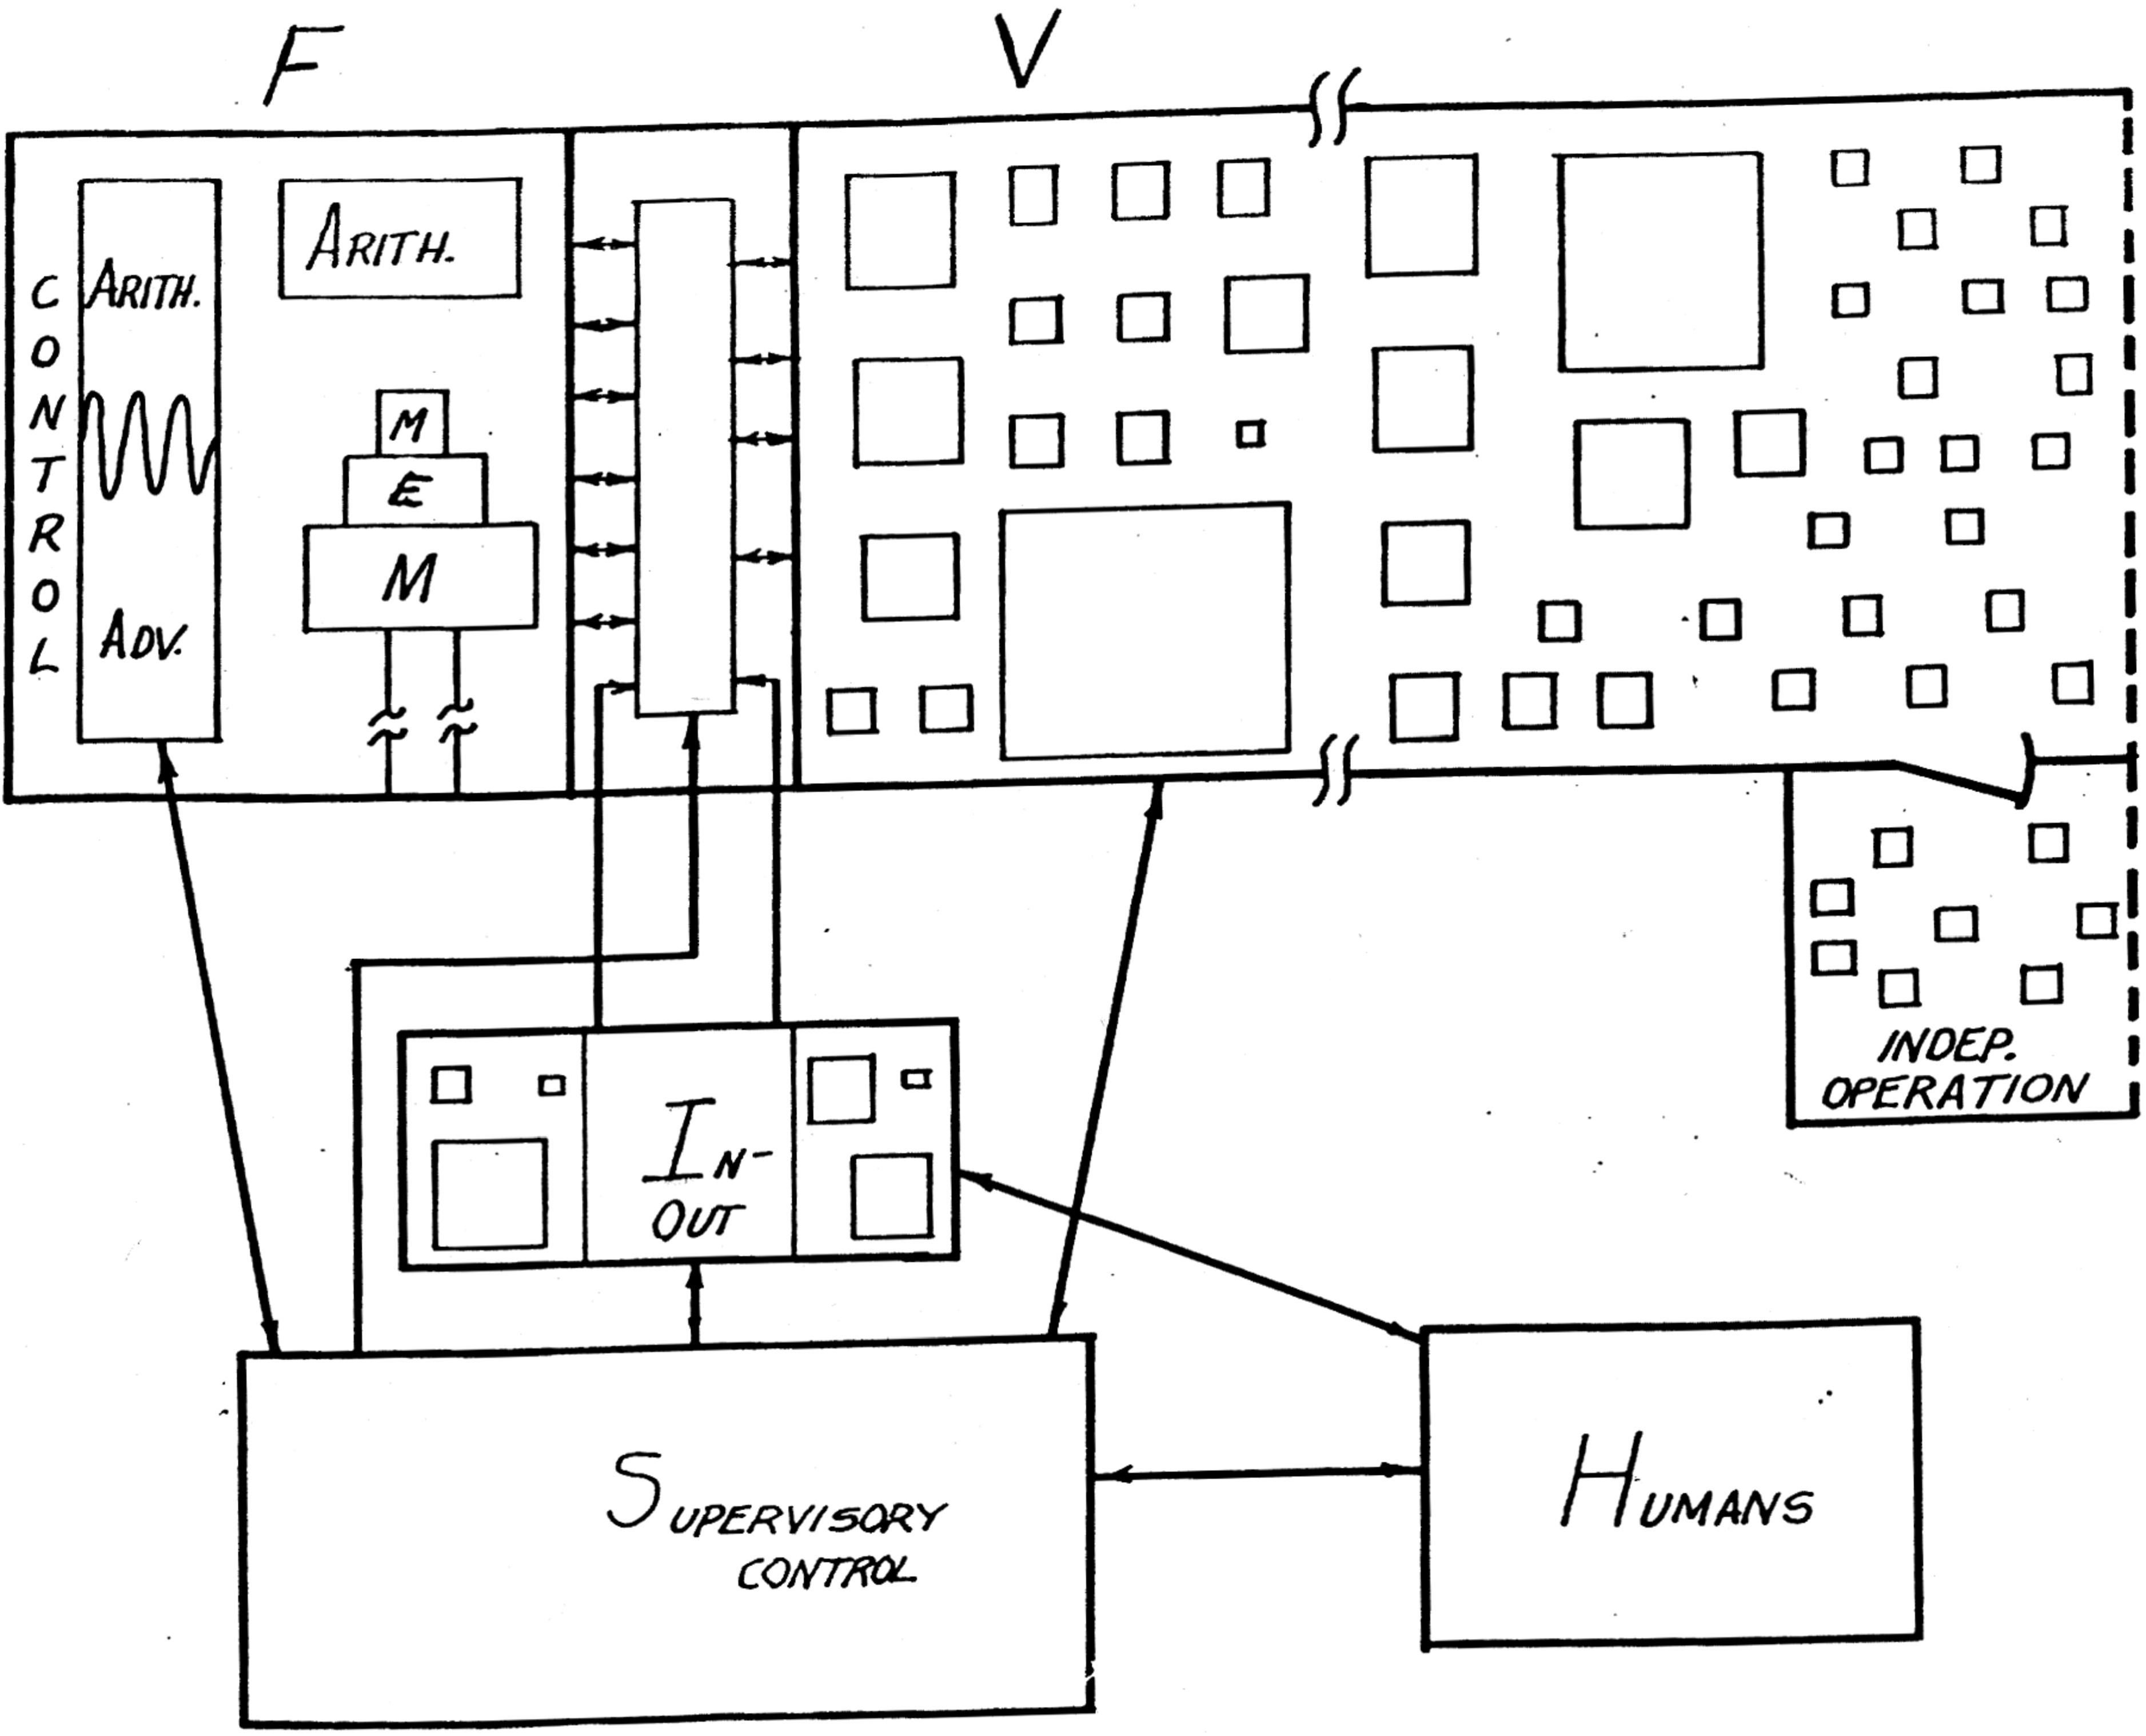
\includegraphics[width=0.7\textwidth]{fig/c1_introducao/model_f+v.pdf}
\caption{Esquem\'atico com o F+V, extraido de \cite{Estrin2002}.}
\label{fig:model_f+v}
\end{figure}

Ao contr\'ario da estrutura F+V proposta por Estrin, a maioria dos sistemas reconfigur\'aveis atuais possuem apenas a parte reconfigur\'avel.
Apesar de sistemas reconfigur\'aveis de alta performance possuirem componentes fixos como processadores e unidades de processamento gr\'aficos (GPUs) \cite{El-Ghazawi2008}, a sua aus\^encia reduz o custo de projeto e a flexibilidade do projeto final.

Os sistemas reconfigur\'aveis atuais utilizam de tr\^es meios principais de programa\c{c}\~ao: \textit{Static Random-Access Memory} (SRAM), \textit{Antifuse} e mem\'orias n\~ao-vol\'ateis.
Usando SRAM, o resultado da s\'i­ntese
%, processo comentado na se\c{c}\~ao \ref{sss:sintese},
 \'e armazenado nas c\'elulas desta mem\'oria e controlam o estado dos transistores das c\'elulas l\'ogicas.
No caso de c\'elulas compostas de tabelas de busca (\textit{look-up tables} ou LUTs), a SRAM armazena os dados dessas c\'elulas.
Outra segunda tecnologia de programa\c{c}\~ao, o \textit{antifuse}, faz uso de uma conex\~ao com imped\^ancia vari\'avel, onde atrav\'es do uso de altas voltagens pode-se modificar a resist\^encia de uma via.
Esse processo de programa\c{c}\~ao \'e irrevers\'i­vel.
As mem\'orias n\~ao vol\'ateis, como EPROM, EEPROM e FLASH, usam transistores especiais com uma ponte flutuante.
Quando a ponte possui carga, o transistor pode ser controlado pela ponte de sele\c{c}\~ao, que permanece carregada at\'e quando desligada.
Estas t\'ecnicas permitem a resist\^encia da \textit{antifuse} e a reprogramabilidade da SRAM, sendo apenas mais complexa e demorada para ser programada \cite{vassiliadis2007fine}.

As interconex\~oes entre c\'elulas l\'ogicas, que logicamente influenciam diretamente as c\'elulas em si, podem ser de cinco tipos: ilha, linha, mar-de-portas, hier\'arquico e estruturas unidimensionais \cite{vassiliadis2007fine}.
A arquitetura do tipo ilha consiste em c\'elulas l\'ogicas conectadas umas as outras atrav\'es de caixas de conex\~oes e de roteamento.
Nesta arquitetura, a c\'elula l\'ogica est\'a cercada por trilhas de conex\~oes, o que explica o nome.
A arquitetura do tipo linha consiste em v\'arias linhas divididas em quantidades variadas de segmentos.
As conex\~oes s\~ao ent\~ao realizadas usando-se linhas verticais atrav\'es de blocos l\'ogicos especiais.
A arquitetura do tipo mar-de-portas consiste de blocos l\'ogicos que cobrem todo o espa\c{c}o do dispositivo e s\~ao conectados aos seus vizinhos diretos.
Em geral este tipo de conex\~ao \'e mais r\'apido.
A arquitetura do tipo hier\'arquico agrupa as c\'elulas l\'ogicas em \textit{clusters}, e agrupa estes em \textit{clusters} de mais alto n\'i­vel, formando de fato um sistema hier\'arquico.
O \'ultimo tipo de arquitetura, unidimensional, surge como uma tentativa de simplificar o roteamento complexo dos sistema bidimensionais apresentados anteriormente.
Nele, restri\c{c}\~oes de aloca\c{c}\~ao e roteamento s\~ao impostas para reduzir o n\'umero de possibilidades.
O problema deste tipo de arquitetura \'e que se n\~ao houverem recursos de roteamento suficientes, o roteamento fica mais complexo que nas arquiteturas bidimensionais.

As arquiteturas reconfigur\'aveis podem ser classificada em tr\^es tipos segundo a granularidade.
A granularidade diz respeito a quantidade de informa\c{c}\~ao m\'i­nima que pode ser passada de uma c\'elula l\'ogica para outra.
Ela separa as arquiteturas reconfigur\'aveis em tr\^es categorias: granularidade fina, grossa e h\'i­brida.
Nas arquiteturas com granularidade fina, como os \textit{Field-Programmable Gate Arrays}, um \'unico \textit{bit} pode ser transferido de uma c\'elula a outra, permitindo assim um maior controle sobre os dados.
Nas arquiteturas com granularidade grossa, os \textit{bits} s\~ao agrupados em palavras de tamanhos fixos, reduzindo assim o espa\c{c}o gasto com roteamento e melhorando a roteabilidade \cite{Hartenstein2001}.
No \'ultimo tipo de arquiteturas, a h\'i­brida, parte das conex\~oes s\~ao grossas e partes s\~ao finas, combinando os benef\'i­cios das duas classes.

%\section{Metodologia}
%\subsection{Fluxo de Projeto}
%\subsubsection{Particionamento}
%\subsubsection{Aloca\c{c}\~ao}
%\subsubsection{S\'i­ntese}
%\label{sss:sintese}

\ifx\compilewholereport\undefined
	\bibliographystyle{authordate1} 
	%\bibliography{bibliografia}
	\newsavebox\mytempbib\savebox\mytempbib{\parbox{\textwidth}{\bibliography{bibliografia}}}
	\listoftodos
	\end{document}
\fi